\documentclass[twocolumn]{article}
\usepackage[a4paper, top=1in, bottom=1in, left=2cm, right=2cm]{geometry}
\usepackage[singlespacing]{setspace}
\usepackage{amsmath}
\usepackage{amssymb}
\usepackage{graphicx}
\usepackage{hyperref}
\usepackage[font=small,labelfont=bf]{caption}
\title{How A Pencil under Water Looks:\\\Large{Utilizing Astroidal Virtual Caustic for the Location of Refraction Image by Flat Boundary}}
\author{M. Ryu \\ {\href{mailto:mingshey@hafs.hs.kr}{mingshey@hafs.hs.kr}}}
\begin{document}
\maketitle
%
%
\section{Introduction}

A pencil partially immersed in water, appearing bent, is a common phenomenon encountered when first learning about refraction (Figure \ref{fig:pencil}). However, the apparent position of the pencil tip varies depending on the viewing angle, a phenomenon that warrants further investigation.

\begin{figure}[ht]
	\centering
	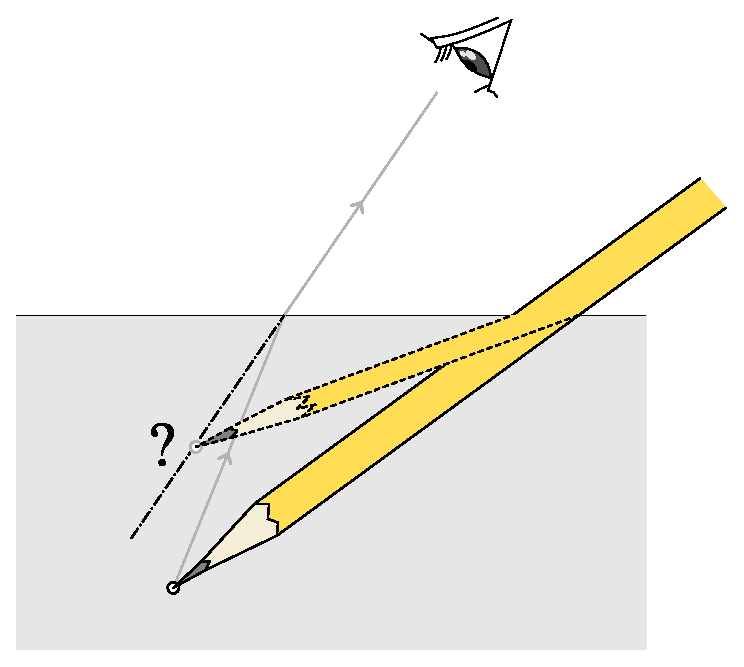
\includegraphics[width=2in]{figs/g164.eps}
	\caption{A pencil appearing bent in water}
	\label{fig:pencil}
\end{figure}

Typically, introductory physics courses cover the apparent depth when viewed vertically. However, a detailed analysis of how the apparent position changes when viewed obliquely is often omitted. Even advanced optics textbooks tend to gloss over this phenomenon, focusing instead on more fundamental topics such as lenses and mirrors.

This is perhaps because a rigorous analysis of this phenomenon requires a level of mathematical sophistication that may be beyond the scope of introductory courses, and its practical applications may be considered less significant compared to the workings of optical instruments. 

However, even seemingly trivial phenomena can sometimes pique our curiosity. It is likely that many others have wondered about this phenomenon as well. This paper aims to provide an answer to this question.


\section{Quick Answer}

For those who are curious but short on time, here's the bottom line: When viewing a point object submerged in water from above, the apparent position of the image varies depending on the point of view. As the viewing point moves, the locus of the observed image on the normal plane forms a type of caustic\footnote{In this case you could call it a \emph{virtual} caustic, since it's the locus of virtual images}, which in this case is a curve known as a \emph{squashed astroid}.

\begin{figure}
	\centering
	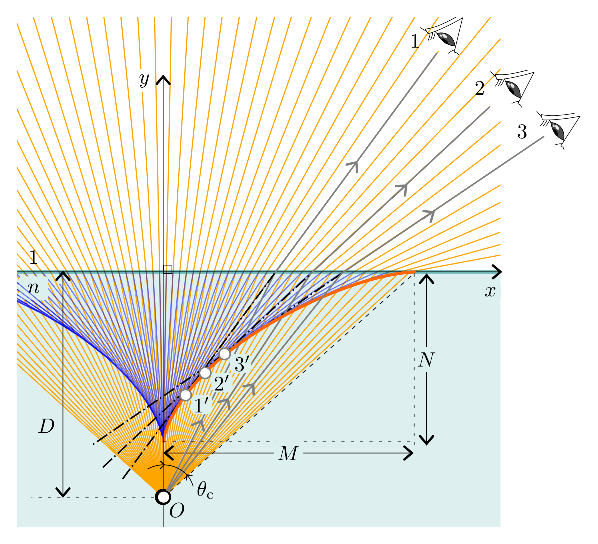
\includegraphics[width=3in]{figs/g409.eps}
	\caption{Locus of the image as the viewpoint moves}
	\label{fig:caustic}
\end{figure}

In the normal plane containing both the object and the viewer, let the intersection of the normal plane and the water surface be the $x$-axis, and the normal line passing through the object be the $y$-axis, as shown in Figure \ref{fig:caustic}. Then, the locus of the image is part of the following curve:

$$ \left| \dfrac{x}{M} \right| ^ {2/3} + \left| \dfrac{y}{N} \right| ^ {2/3} = 1,$$
where $M = D/\sqrt{n^2 - 1}$ is the maximum incident distance determined by the critical angle of total internal reflection ($\theta_{\mathrm{c}}$), $N = D/n$ is the apparent depth when viewed directly from above, $D$ is the actual depth of the object, and $n$ is the refractive index of water relative to air.

\section{Derivation of the Equation}

Let $n_1$ and $n_2$ be the refractive indices of air and water, respectively. A point object $\mathrm{O}$ is located at a depth $D$ below the air-water interface. A ray of light emanating from the object is incident on point $\mathrm{A}$ on the interface, which is a distance $a$ from the $y$-axis, at an angle of $\theta_2$ to the normal. The ray is then refracted into the air at an angle of $\theta_1$ to the same normal.

The extension of the refracted ray intersects the $y$-axis at point $\mathrm{B}(0, b)$. As the angle of incidence $\theta_2$ varies, the lines AB envelope a curve, which is defined as the caustic curve. Note that in this case, the caustic is a virtual caustic formed by the extensions of the rays, rather than the rays themselves. The image is located at point $\mathrm{C}$, the point of tangency between the line segment AB and the caustic. This is because the bundle of rays near this point diverges locally.

\begin{figure}
	\centering
	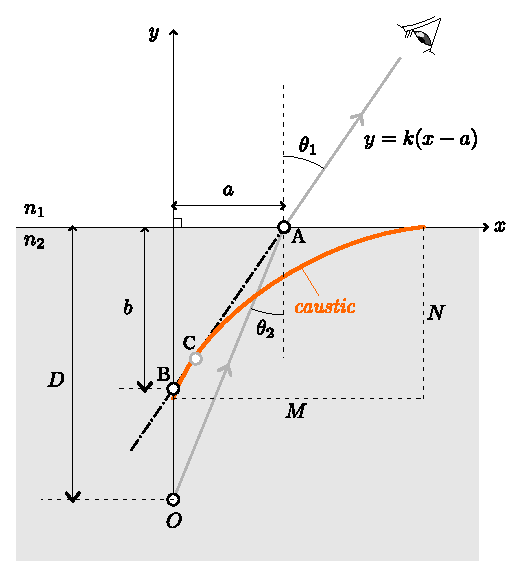
\includegraphics[width=3in]{figs/g237.eps}
	\caption{Light rays and the caustic.}
	\label{fig:geometry}
\end{figure}

The straight line $\mathrm{AB}$ can be expressed by the following equation, where $a$ is the distance from the $y$-axis to the point of incidence:
$$y=k(x-a).$$

Considering Snell's law, $ {n_1} \sin\theta_1 = {n_2} \sin\theta_2$, or $ \sin\theta_1 = n\sin\theta_2,$
the slope of the line, $k$, is given by
$$k=\dfrac{1}{\tan\theta_1}=\dfrac{\cos\theta_1}{\sin\theta_1}
=\dfrac{\sqrt{1-n^2\sin^2\theta_2}}{n\sin\theta_2}.$$

Geometrically, the following relationships hold:
$$\begin{aligned}
	a &= D\tan\theta_2 = \frac{D\sin\theta_2}{\cos\theta_2},\\
	b &= -ka \\
	&= -\frac{D\sin\theta_2}{\cos\theta_2} \cdot \frac{\sqrt{1-n^2\sin^2\theta_2}}{n\sin\theta_2}\\
	&= -\frac{D\sqrt{1-n^2\sin^2\theta_2}}{n\cos\theta_2}.
\end{aligned}$$

Introducing dimensionless parameters $\alpha = a/M$ and $\beta = b/N$, we have

\begin{equation}
	\begin{aligned}
		\alpha^2 + \beta^2 &= \frac{a^2}{M^2} + \frac{b^2}{N^2} \\
		&= \frac{n^2-1}{D^2} \frac{D^2\sin^2\theta_2}{\cos^2\theta_2} + \frac{n^2}{D^2} \frac{D^2(1-n^2\sin^2\theta_2)}{n^2\cos^2\theta_2} \\
		&= \frac{(n^2-1)\sin^2\theta_2 + 1-n^2\sin^2\theta_2}{\cos^2\theta_2} \\
		&= \frac{1-\sin^2\theta_2}{\cos^2\theta_2} \\
		&= 1
	\end{aligned}
\end{equation}

Now, let's introduce dimensionless coordinates $\xi = x/M$ and $\eta = y/N$. As the viewpoint moves in the $xy$-plane, points $\mathrm{A}(a, 0)$ and $\mathrm{B}(0, b)$ also move. The corresponding points $\mathrm{A'}(\alpha, 0)$ and $\mathrm{B'}(0, \beta$) move in the $\xi\eta$-plane maintaining a constant distance of $1$.

\begin{figure}[!t]
	\centering
	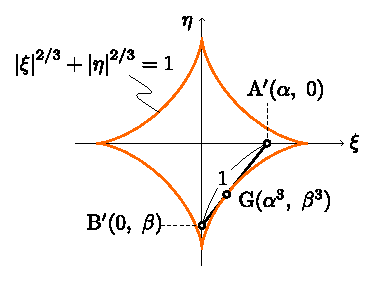
\includegraphics[width=2.5in]{figs/g107.eps}	
	\caption{Projection of the caustic onto the $\xi\eta$ plane, revealing an astroid shape.}
	\label{fig:astroid}
\end{figure}

The envelope of the family of lines ${\mathrm{A'B'}}$ parameterized by $\alpha$ is a well-known curve called an \emph{astroid}\footnote{Not to be confused with the \emph{asteroid} meaning a small celestial body.}, which can be described by the equation:
$$ \left| \xi \right|^{2/3} + \left| \eta \right|^{2/3} = 1. $$
(See Appendix \ref{app:astroid} for details.)

The point of tangency between the line ${\mathrm{A'B'}}$ and the astroid is $\mathrm{G}(\alpha^3, \beta^3)$, which corresponds to the image point $\mathrm{C}$.

Therefore, the coordinates of the image point $(x_{\mathrm{C}}^{}, y_{\mathrm{C}}^{})$ can be obtained from the following relations:
$$
\left\{
\begin{aligned}
	\xi_G &= \dfrac{x_C}{M} = \alpha^3 = \dfrac{a^3}{M^3},\\
	\eta_G &= \dfrac{y_C}{N} = \beta^3 = \dfrac{b^3}{N^3}.
\end{aligned}
\right.
$$
That is,
$$
\left\{
\begin{aligned}
	x_C &= \dfrac{a^3}{M^2},\\
	y_C &= \dfrac{b^3}{N^2}=-\dfrac{k^3a^3}{N^2}.
\end{aligned}
\right.
$$

Using 
$\sin\theta_2 = {a}/{\sqrt{D^2+a^2}}$
we obtain
$$k = \dfrac{\sqrt{D^2-(n^2-1)a^2}}{na},$$
and the position of the image can be expressed as parametric functions of $a$:
$$ \left\{ 
\begin{aligned}
	x_{\mathrm{C}}^{} &= (n^2-1)\dfrac{a^3}{D^2},\\
	y_{\mathrm{C}}^{} 
	%	&= -\dfrac{n^2}{D^2}\dfrac{a^3}
	%	{n^3a^3}\left\{ D^2-(n^2-1)a^2 \right\}^{3/2}\\
	&=-\dfrac{D}{n}\left\{ 1-(n^2-1)\dfrac{a^2}{D^2} \right\}^{3/2}.
\end{aligned}
\right.$$

\section{When the viewpoint is submerged in water}

When an object is in air at a height $D$ above the boundary, and the viewer is in water, the relative refractive index is $1/n < 1$. By similar reasoning, we obtain the following equation for the caustic (see Appendix \ref{app:hyperastroid}):
$$ \left| \xi \right|^{2/3} - \left| \eta \right|^{2/3} = -1, $$
where $\xi = {x}/{W} $ and $\eta = {y}/{Z}$, with $W = {nD}/{\sqrt{n^2-1}}$ and $Z = nD$. 
Although this curve does not have asymptotes, its slope converges to $\pm Z/W = \pm \sqrt{n^2-1}$ as $x \to \pm\infty$.

\begin{figure}
	\centering
	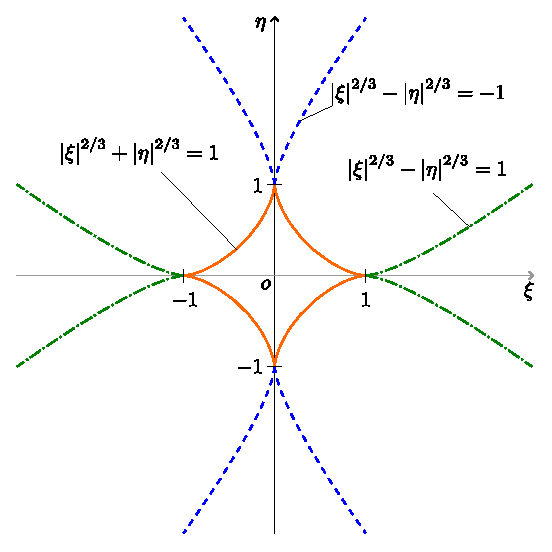
\includegraphics[width=3in]{figs/g254.eps}
	\caption{Astroid and `\emph{hyperastroids}'}
	\label{fig:hyperastroid}
\end{figure}

Thus, the skyscape viewed from underwater appears compressed within a circle (or cone) centered on the vertical axis and bounded by the critical angle for total internal reflection. This phenomenon is well-known as \emph{Snell's window} and it gives field of view  similar to that of a \href{https://en.wikipedia.org/wiki/Fisheye_lens}{fisheye lens} used in ultra wide-angle photography.

A more general form of this curve is the family of curves defined by
$$ \left| \xi \right|^{r} - \left| \eta \right|^{r} = \pm 1, $$
which is referred to as \emph{Super Hyperbola} by \href{http://dynamicmathematicslearning.com/super-ellipse.html}{DML}\footnote{\ttfamily{dynamicmathematicslearning.com/super-ellipse.html}} and is included in a broader family of curves called \emph{superconics} along with the family of curves called \emph{superellipse} which is defined by
$$ \left| \xi \right|^{r} + \left| \eta \right|^{r} = 1, $$ 
as defined in the  \href{https://old.nationalcurvebank.org/superconicncb/superconicncb.htm}{`National Curve Bank'}%
\footnote{\ttfamily{old.nationalcurvebank.org/superconicncb/\\superconicncb.htm}}, to which astroid belongs.

In particular, for the special case where $r = 2/3$, the resulting curve
$$ \left| \xi \right|^{2/3} - \left| \eta \right|^{2/3} = \pm1, $$
has physical significance as the caustic of light rays emanating from a point source in the air and refracted into the water. Moreover, the relationship between this curve and the astroid is analogous to that between a hyperbola and an ellipse, suggesting the name \emph{hyperastroid}. 

\section{Finding the Image Position}

Given the position of an object and the viewpoint, the image position can be determined using the caustic as follows.

\begin{figure}[!h]
	\centering
	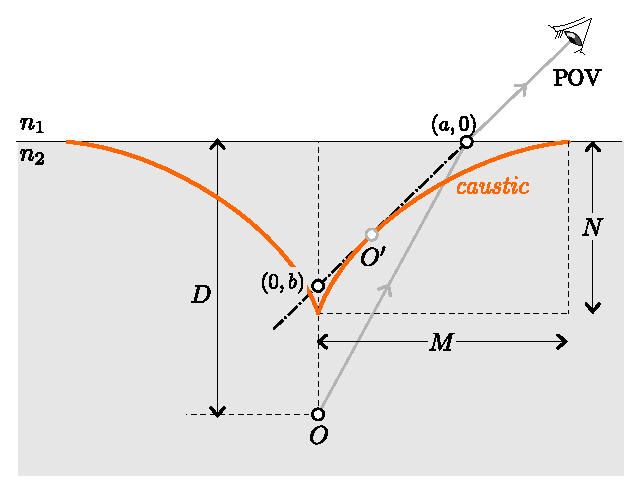
\includegraphics[width=2.7in]{figs/g394.eps}
	\caption{Determining the image position using the caustic}
	\label{fig:image_caustic}
\end{figure}

As shown in Figure \ref{fig:image_caustic}, a tangent line is drawn from the viewpoint (POV) to the caustic. The point of tangency ($\mathrm{O'}$) on the caustic is the image position, and the intersection point of the tangent line with the water surface is the point where the light ray from the object ($\mathrm{O}$) enters the interface with air.

Let $(x_{\mathrm{V}}, y_{\mathrm{V}})$ be the coordinates of the viewpoint (POV), $(x_{\mathrm{O}}, y_{\mathrm{O}})$ of the object ($\mathrm{O}$), and $(x_{\mathrm{O'}}, y_{\mathrm{O'}})$ of the image ($\mathrm{O'}$) that we want to find. Let A and B be the points where the extension of the refracted ray intersects the water surface and the normal line passing through O (which is the $y$-axis), with coordinates $(a, 0)$ and $(0, b)$, respectively. 

In the $\xi\eta$ coordinate system, the corresponding points are, the viewpoint: $(\xi_{\mathrm{V}}, \eta_{\mathrm{V}})=(x_{\mathrm{V}}/M, y_{\mathrm{V}}/N)$, the object: $(\xi_{\mathrm{O}}, \eta_{\mathrm{O}})=(x_{\mathrm{O}}/M, y_{\mathrm{O}}/N)$, and the image: $(x_{\mathrm{O'}}/M, y_{\mathrm{O'}}/N)=(\alpha^3, \beta^3)$, while the coordinates of $\mathrm{A'}$ and $\mathrm{B'}$ are $(\alpha, 0)=(a/M, 0)$ and $(0, \beta)=(0, b/N)$, respectively. Here, $M=D/\sqrt{n^2-1}$, $N=D/n$, and $D=y_{\mathrm{O}}$. 

From the proportional relationship between the tangent, the water surface, and the $\eta$-axis, we obtain the following equation:
$$\dfrac{\eta_{\mathrm{V}}}{\xi_{\mathrm{V}}-\alpha}=-\dfrac{\beta}{\alpha}.$$
Using $\beta = \pm \sqrt{1-\alpha^2}$ and squaring both sides, we obtain the following quartic equation for $\alpha$:
\[
\left( 1 - \alpha^2 \right) \left(\alpha-\xi_{\mathrm{V}} \right)^2 = \alpha^2 \eta_{\mathrm{V}}^2
\]
Generally, a quartic equation has four complex roots, and in this case, there are two real roots. The desired value of $\alpha$ is the one between 0 and $\xi_{\mathrm{V}}$. Solving a quartic equation manually is generally difficult. Although an analytical solution can be obtained using a computer algebra system (CAS), it is often more efficient to find an approximate solution using numerical methods. (See Appendix \ref{app:python})

As can be seen from the form of the equation, the location of the image depends on that of the viewpoint. For example, as shown in Figure \ref{fig:pencil_view}, the tip of a partially submerged pencil appears at different positions, $1'$ and $2'$, when viewed from points $1$ and $2$, respectively.

\begin{figure}[h]
	\centering
	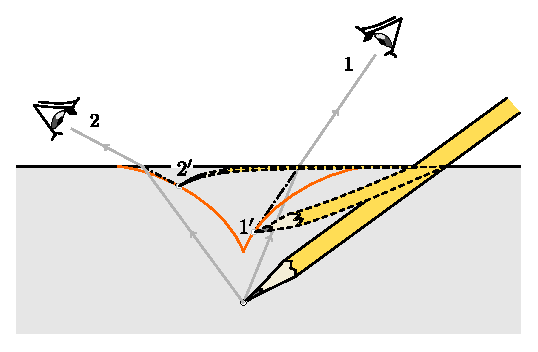
\includegraphics[width=2.4in]{figs/g43.eps}
	\caption{Image of a pencil partially submerged in water. The image of the pencil tip moves from $1'$ to $2'$ as the viewpoint changes from $1$ to $2$.}
	\label{fig:pencil_view}
\end{figure}

If there is a continuous object in water, as shown in Figure \ref{fig:extended_image}, we can find the corresponding image points $1', 2', 3', \dots$ for points $1, 2, 3, ...$ on the object using the same method. The locus of these image points, as the points move continuously, forms the image of the object.

\begin{figure}[h]
	\centering
	\includegraphics*[width=2.5in]{figs/g242.eps}
	\caption{Image of a continuous object. By connecting the image points $1', 2', 3', \dots$ corresponding to points $1, 2, 3, \dots$ on the object, the overall shape of the image can be drawn.}
	\label{fig:extended_image}
\end{figure}

\begin{figure}[!h]
	\centering
	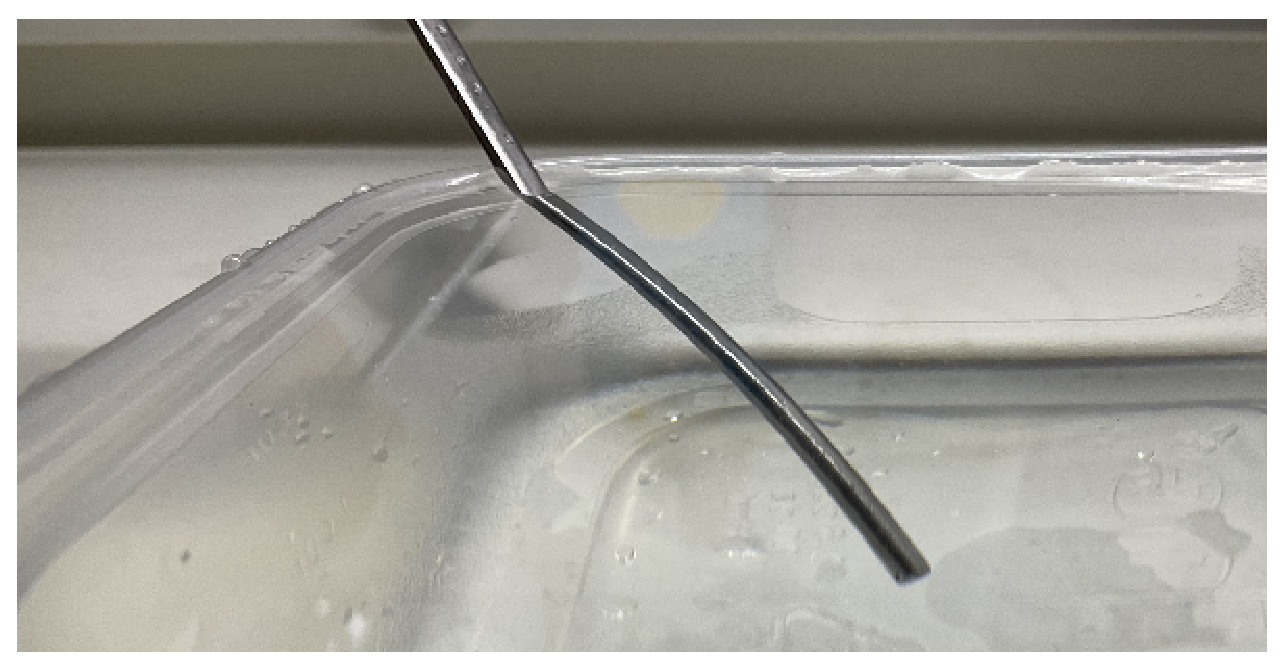
\includegraphics[width=3in]{figs/img_1805_2.eps}
	\caption{Photograph of a chopstick partially submerged in water. Taken from a low angle close to the water surface.}
	\label{fig:picture}
\end{figure}

Another approach is to determine the intersection point of the ray with the water surface by solving the equation
\[
\dfrac{n_1 \left( x - x_{\mathrm{V}}^{} \right)}{\sqrt{ y_{\mathrm{V}}^2 + \left( x - x_{\mathrm{V}}^{} \right)^2 }}
+\dfrac{n_2 \left( x - x_{\mathrm{O}}^{} \right)}{\sqrt{ y_{\mathrm{O}}^2 + \left( x - x_{\mathrm{O}}^{} \right)^2 }}
= 0,
\]
or after rearranging,
\[ \begin{aligned}
	\left( x - x_{\mathrm{V}}^{} \right)^2 &\left\{ y_{\mathrm{V}}^2 + \left(x - x_{\mathrm{V}}^{} \right)^2 \right\} \\
	&= n^2 \left( x - x_{\mathrm{O}}^{} \right)^2 \left\{ y_{\mathrm{V}}^2 + \left(x - x_{\mathrm{V}}^{} \right)^2 \right\},
\end{aligned}
\]
which is obtained by applying Fermat's principle. The abscissa of the intersection point, which is a real root of the quartic equation
lying between $x_{\mathrm{O}}^{}$ and $x_{\mathrm{V}}^{}$, can then be used to determine the image position using the equation of the tangent point of the astroid.

As in the tangent approach, numerical methods can be more efficient than analytical methods for practical purposes. A Python example demonstrating how to find the image position using both analytical and numerical methods can be found at 
\href{https://github.com/mingshey/python_projects/blob/main/Refraction_Image.ipynb}%
{\sffamily{github}}\footnote{\ttfamily{https://github.com/mingshey/python\_projects/blob/main/\\Refraction\_Image\_en.ipynb}}

\section{Image of the Submerged Space}

Having established a quantitative method to locate the image, let's investigate how the overall appearance of the submerged space is distorted when viewed from above the water. As shown in Figure \ref{fig:grid_underwater}, a rectangular region in water represented by a square grid appears as shown in Figures \ref{fig:image_underwater} to \ref{fig:seashell} depending on the relative height of the viewpoint.

\begin{figure}
	\centering
	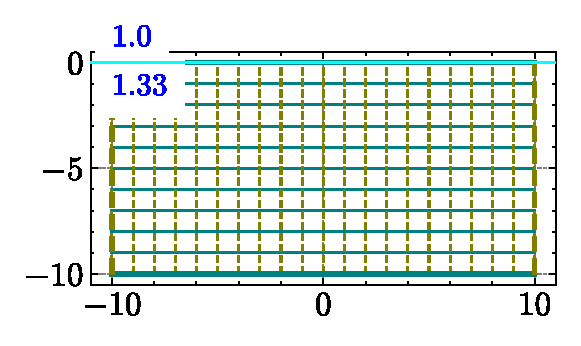
\includegraphics[width=2.5in]{figs/grid_underwater.eps}
	\caption{A grid-shaped object placed underwater}
	\label{fig:grid_underwater}
\end{figure}

\begin{figure}[!t]
	\centering
	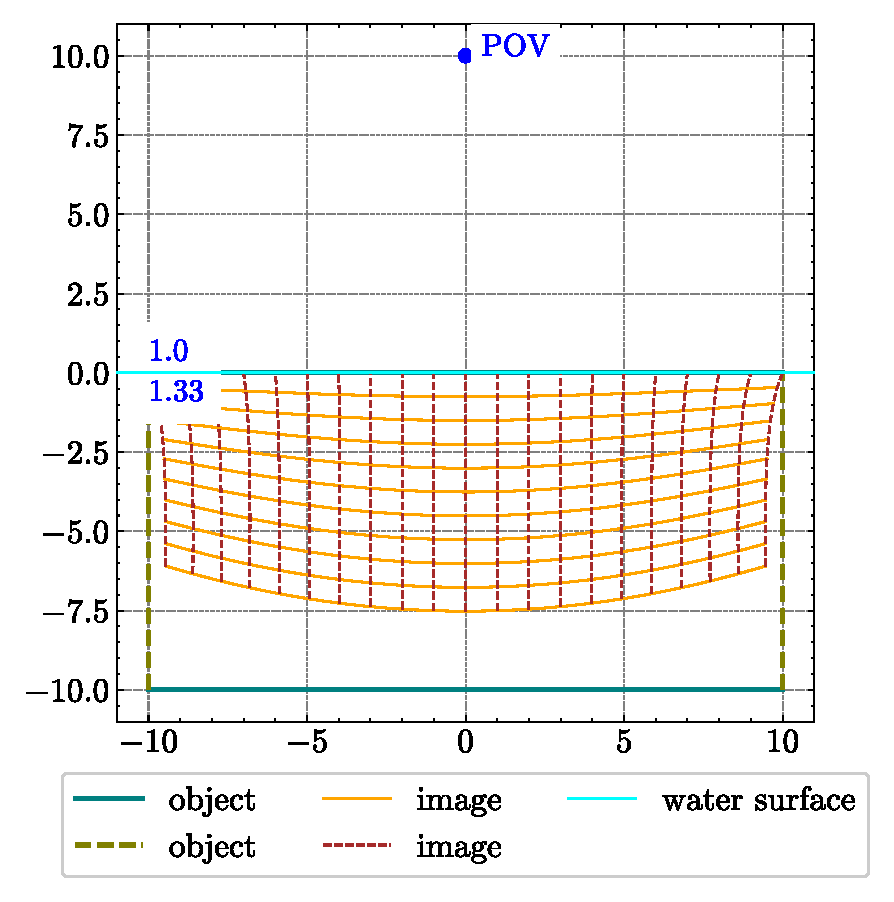
\includegraphics[width=3in]{figs/image_underwater1.eps}
	\caption{Image of the grid. When the viewer's eye level is similar to or higher than the water depth, the image appears to be flattened overall in a ratio approximately equal to the refractive index.\\
	The outline of the grid is shown as a rectangle for comparison in \ref{fig:image_underwater}$\sim$\ref{fig:snell_window}}
	\label{fig:image_underwater}
\end{figure}

\begin{figure}[!t]
	\centering
	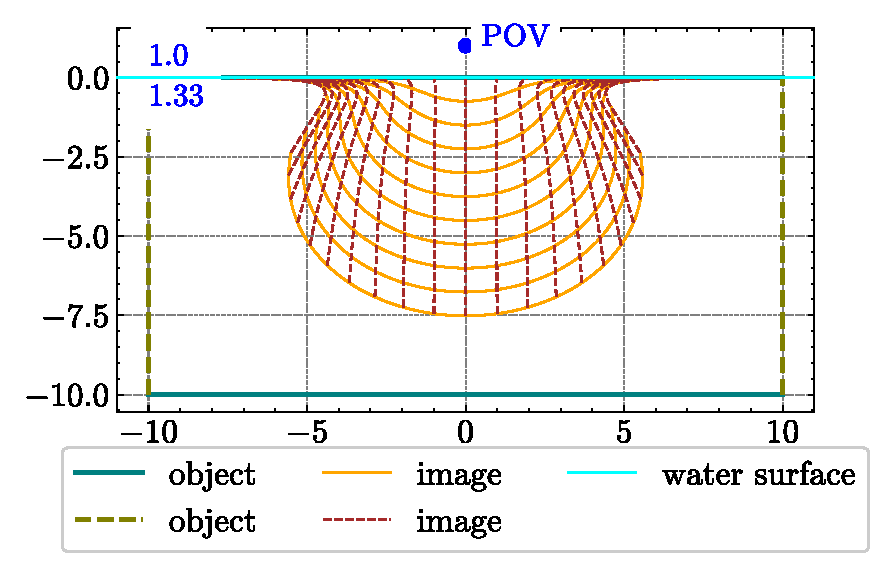
\includegraphics[width=3in]{figs/fishjar.eps}
	\caption{Image of the grid. When the viewer's eye level is much lower than the water depth, the rectangular space appears compressed into a fishbowl shape.}
	\label{fig:fishbowl}
\end{figure}

\begin{figure}[!t]
	\centering
	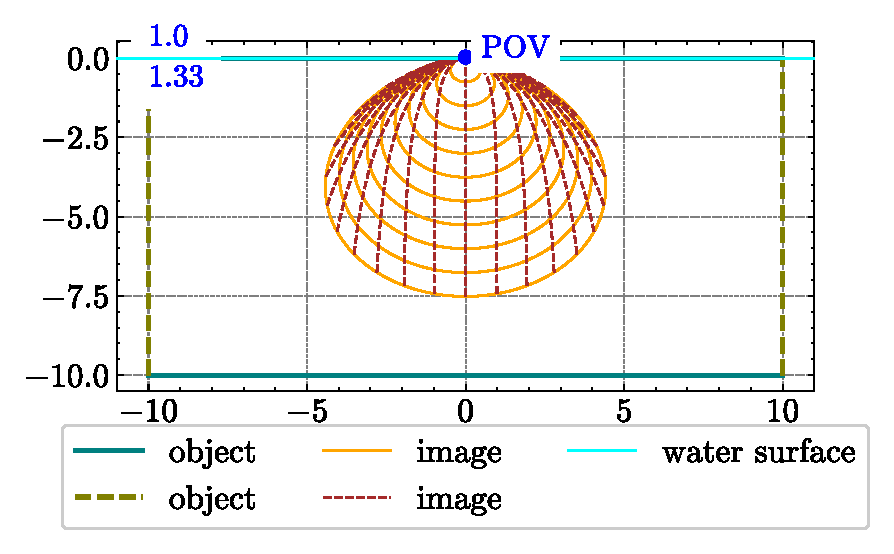
\includegraphics[width=3in]{figs/seashell_shape.eps}
	\caption{Image of the grid. When the viewer's eye is extremely close to the water surface, the rectangular space appears compressed into a shape resembling a seashell.}
	\label{fig:seashell}
\end{figure}

\begin{figure}[!h]
	\centering
	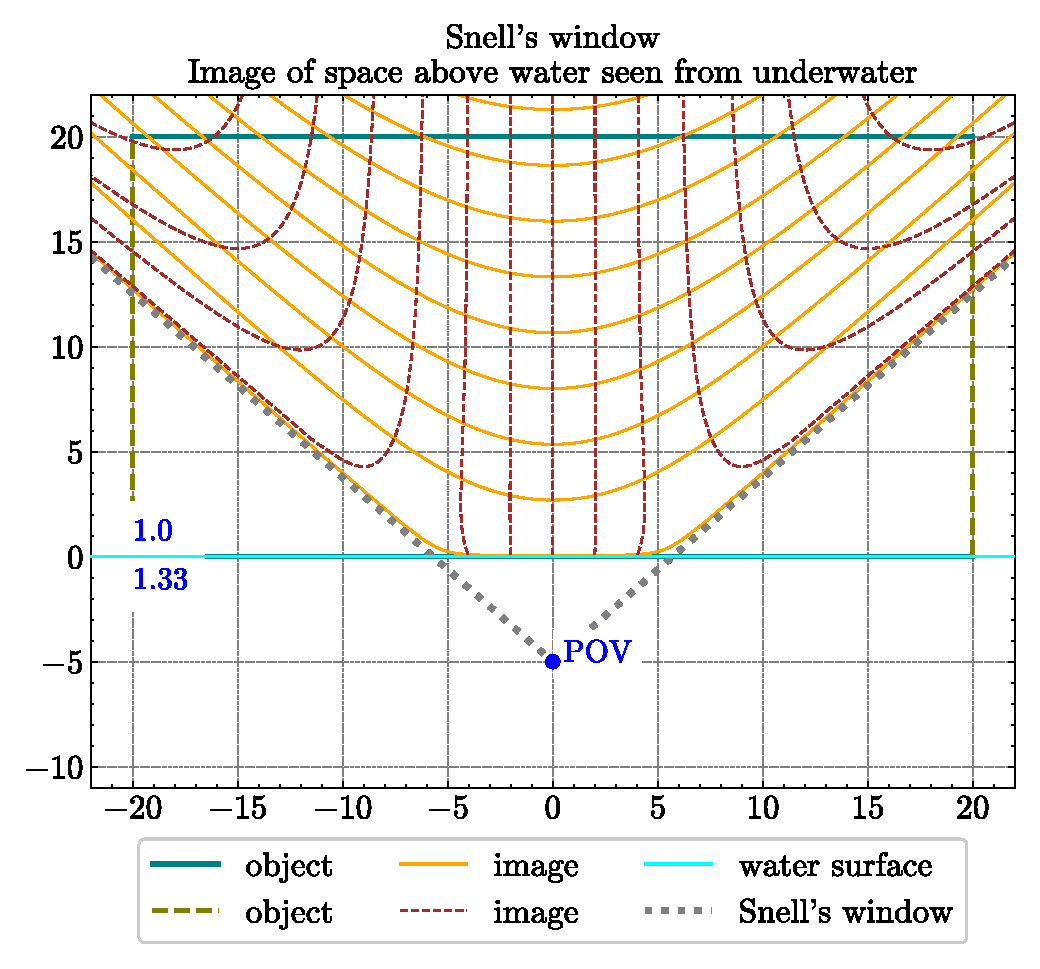
\includegraphics[width=3.3in]{figs/snell_window.eps}
	\caption{Snell's window. The appearance of an object viewed from underwater. The generating line of the cone defining Snell's window is conveniently denoted as Snell's window.}
	\label{fig:snell_window}
\end{figure}

When a grid of equal squares is placed in the air adjacent to the water surface, the apparent shape of the grid viewed from underwater is compressed within a cone bounded by the critical angle of total internal reflection, as shown in Figure \ref{fig:snell_window}. The circle where the water surface intersects this cone is called Snell's window, and the entire sky above the water surface appears compressed within this window. The space directly above Snell's window is relatively undistorted and appears to be magnified by a factor equal to the refractive index ratio, while other regions appear distorted with compressed visual angles and increased perceived distances. The distortion is particularly noticeable near the water surface.



\appendix
\section*{Appendices}
\section{The Astroid Defined as an Envelope} \label{app:astroid}
Consider two points in the Cartesian plane: $(a, 0)$ on the $x$-axis and $(0, b)$ on the $y$-axis. Suppose these points maintain a constant distance $c$ from each other. Then, we have $a^2 + b^2 = c^2$, and the equation of the line connecting these two points at any given moment is given by
$$y = -\frac{b}{a}(x-a)$$
Substituting $b = \pm \sqrt{c^2 - a^2}$ yields
$$y(x, a) = \mp \frac{\sqrt{c^2 - a^2}}{a}(x-a)$$
As the value of a varies, the line connecting the two points also varies. The envelope of this family of lines can be defined as the locus of points that remain stationary as a undergoes an infinitesimal change, i.e., points where
$$\frac{\partial y}{\partial a} = 0.$$
Differentiating y with respect to a, we obtain
$$
\begin{aligned}
	\frac{\partial y}{\partial a} &= \pm\left[\left( \frac{1}{\sqrt{c^2-a^2}}+\frac{\sqrt{c^2-a^2}}{a^2}\right) (x-a) + \frac{\sqrt{c^2-a^2}}{a} \right]\\
	&= \pm \frac{(a^2+c^2-a^2)(x-a)+a(c^2-a^2)}{a^2\sqrt{c^2-a^2}}\\
	&= \pm \frac{c^2 x - a^3}{a^2 \sqrt{c^2 - a^2}}\\
	&= 0.
\end{aligned}
$$
Therefore, the $x$-coordinate of the stationary point is $x = a^3/c^2$. Substituting this into $y(x, a)$, we obtain the $y$-coordinate:
$$
\begin{aligned}
	y(x, a) &= \mp \frac{\sqrt{c^2-a^2}}{a}\left(\frac{a^3}{c^2}-a\right)\\
	& = \pm \frac{\left( c^2- a^2 \right)^{3/2}}{c^2}\\
	& = \frac{b^3}{c^2}
\end{aligned}
$$
Therefore, the coordinates of the stationary point $(x, y)$ satisfy the equation of the astroid:
$$ \left|\dfrac{x}{c}\right|^{2/3} + \left|\dfrac{y}{c}\right|^{2/3} = 1. $$

\section{Hyperbolic Astroid} \label{app:hyperastroid}
We define a 'hyperbolic astroid' as the envelope of the line segment connecting points A$(a, 0)$ on the $x$-axis and B$(0, b)$ on the $y$-axis, where these points satisfy the relation:
$b^2-a^2=c^2$
The equation of this envelope is given by the following hyperbolic astroid equation:
$$ \left|\dfrac{x}{c}\right|^{2/3} - \left|\dfrac{y}{c}\right|^{2/3} = -1. $$
The derivation is similar to that in Appendix \ref{app:astroid} and is omitted here.
If we draw a tangent line from a point A to the envelope, the coordinates of the tangent point are given by $(-a^3/c^2, b^3/c^2)$. 
If we draw a tangent line from an arbitrary point $(x_{\mathrm{V}^{}}, y_{\mathrm{V}}^{})$ to the hyperbolic astroid, and let $(a,0)$ be the point where the tangent line intersects the $x$-axis, then $a$ is a real root of the quartic equation
$$ \left( a^2 + c^2 \right) \left(a - x_{\mathrm{V}}^{} \right)^2 = a^2 y_{\mathrm{V}}^2$$
lying between $0$ and $x_{\mathrm{V}^{}}$, and $b = \pm \sqrt{a^2 + c^2}$.

\section{Python Code for Finding the Image Location Using the Tangent to the Astroid} \label{app:python}
\begin{verbatim}
	import numpy as np
	import sympy as sym
	from scipy.optimize import root
	
	ksi, eta, alfa = sym.symbols('xi eta alpha')
	eqn = (alfa - ksi)**2 * (1 - alfa**2)\
	- alfa**2 * eta**2
	eqnf = sym.lambdify((ksi, eta, alfa), eqn);
	
	def imgloc(pov, obj, nrel):
	xv, yv = pov
	xo, yo = obj
	M = yo / np.sqrt(nrel**2 - 1)
	N = yo / nrel
	xi_v = (xv - xo) / M
	eta_v = yv / N
	alpha = root(lambda x:\
	eqnf(xi_v, eta_v, x), xi_v).x[0]
	beta = np.sqrt(1 - alpha**2)
	xim = alpha**3 * M + xo
	yim = beta**3 * N
	xpoi = (xim*yv - yim*xv)/(yv - yim)
	
	img = np.array([xim, yim])
	poi = np.array([xpoi, 0])
	
	return img, poi
\end{verbatim}

\vfill
\section*{}
\slshape{This document is translated from original Korean with the assistance of Google's Gemini language model.}
\end{document}